
As more data becomes available to the model, the posterior density for $p$ increases near the expected value (i.e., we become more certain about the value of $p$). See Figure \ref{figure:iterative_posterior}. 

\begin{figure}[H]
    \centering
    \begin{subfigure}[t]{0.4\textwidth}
        \centering
        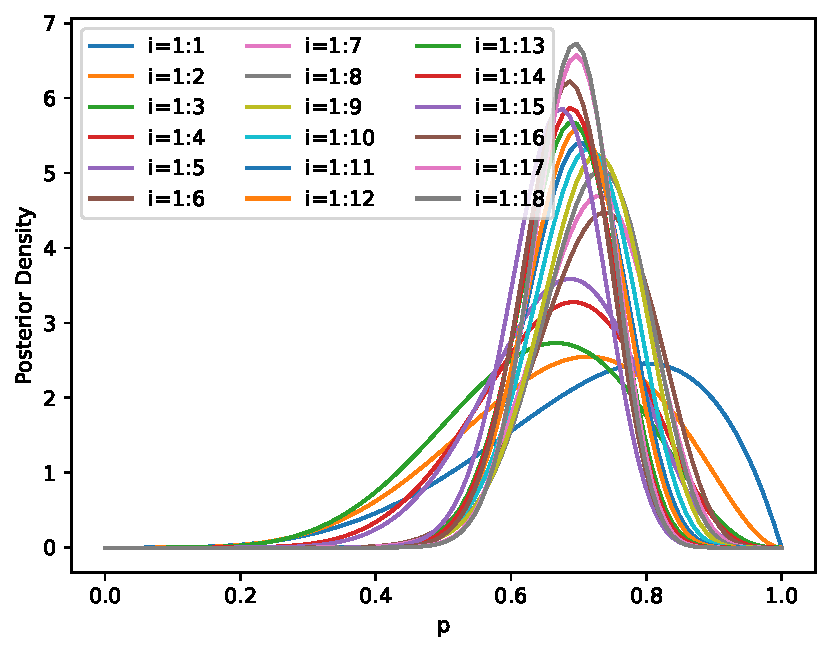
\includegraphics[width=\textwidth]{images/bnb_iterative_posterior.pdf}
        \caption{Posterior distribution as each new value of $X$ is added.}
    \end{subfigure}
    \begin{subfigure}[t]{0.4\textwidth}
        \centering
        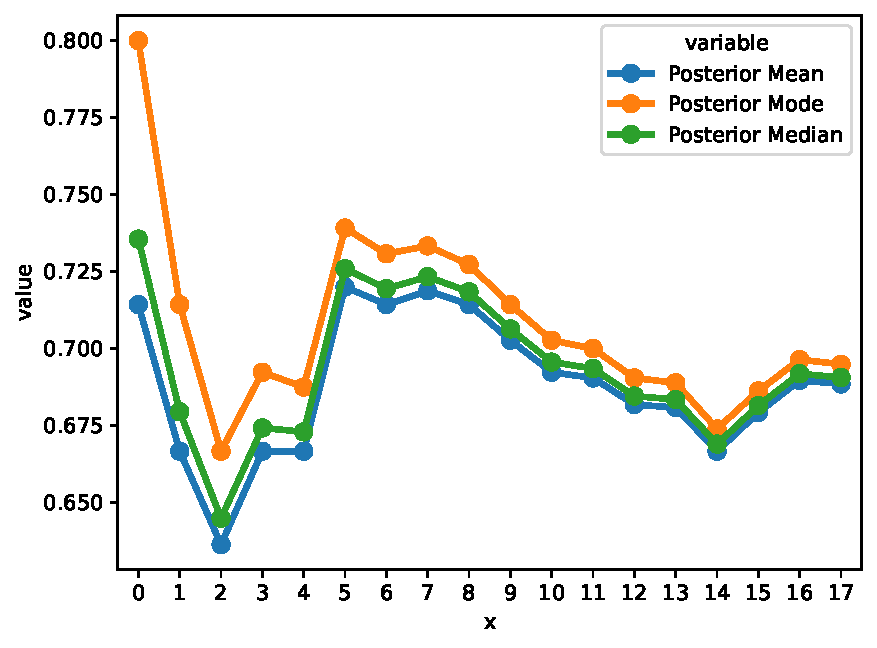
\includegraphics[width=\textwidth]{images/iterative_posterior_summaries.pdf}
        \caption{Posterior summaries for models as each new value of X is added.}
    \end{subfigure}
    \caption{}
    \label{figure:iterative_posterior}
\end{figure}